% The difference table of k^3: the leading entries 0, 1, 6, 6 are the coefficients of k^3 in the binomial basis. Generated by figs_t0c01.py.
\begin{tikzpicture}[x=1.05cm,y=0.75cm]
\node[font=\small,anchor=east] at (-0.6,0) {$P(k)=k^3$};
\node[draw=BrickRed,fill=BrickRed!12,rounded corners=2pt,inner sep=2pt,font=\small] at (0.00,0) {$0$};
\node[font=\small] at (1.00,0) {$1$};
\node[font=\small] at (2.00,0) {$8$};
\node[font=\small] at (3.00,0) {$27$};
\node[font=\small] at (4.00,0) {$64$};
\node[font=\small] at (5.00,0) {$125$};
\node[font=\small,anchor=east] at (-0.6,-1) {$\Delta P$};
\node[draw=BrickRed,fill=BrickRed!12,rounded corners=2pt,inner sep=2pt,font=\small] at (0.50,-1) {$1$};
\node[font=\small] at (1.50,-1) {$7$};
\node[font=\small] at (2.50,-1) {$19$};
\node[font=\small] at (3.50,-1) {$37$};
\node[font=\small] at (4.50,-1) {$61$};
\node[font=\small,anchor=east] at (-0.6,-2) {$\Delta^2P$};
\node[draw=BrickRed,fill=BrickRed!12,rounded corners=2pt,inner sep=2pt,font=\small] at (1.00,-2) {$6$};
\node[font=\small] at (2.00,-2) {$12$};
\node[font=\small] at (3.00,-2) {$18$};
\node[font=\small] at (4.00,-2) {$24$};
\node[font=\small,anchor=east] at (-0.6,-3) {$\Delta^3P$};
\node[draw=BrickRed,fill=BrickRed!12,rounded corners=2pt,inner sep=2pt,font=\small] at (1.50,-3) {$6$};
\node[font=\small] at (2.50,-3) {$6$};
\node[font=\small] at (3.50,-3) {$6$};
\node[font=\small,anchor=east] at (-0.6,-4) {$\Delta^4P$};
\node[draw=BrickRed,fill=BrickRed!12,rounded corners=2pt,inner sep=2pt,font=\small] at (2.00,-4) {$0$};
\node[font=\small] at (3.00,-4) {$0$};
\node[font=\small,anchor=north,text width=7cm,align=center] at (3,-4.6) {$k^3=0\binom k0+1\binom k1+6\binom k2+6\binom k3$};
\end{tikzpicture}
